\chapter{Analysis}\label{cha:Analysis}
% \section{Analysis}

Different non-invasive approaches for leaf disease detection have been developed, and the application of Machine learning algorithms on image datasets from various sensors are gaining traction \cite{ferentinos2018deep, ahmed2019rice, annabel2019machine, ramesh2018plant}. A typical learning-based approach workflow consists of input datasets acquisition, data pre-processing, model training, model evaluation and finally, deployment. Feature extraction, segmentation, and region detection are data pre-processing steps for image datasets. This chapter starts with a brief explanation of the Convolutional Neural Network (CNN) in deep learning in section \ref{sec:machinedeep}. Then, the paper further reviews different machine learning and deep learning techniques used in research papers to detect different diseases in sugar beet leaves in section \ref{sec:deeplapproach} and \ref{sec:machineapproach}, respectively.

% ✅✅✅
\section{Machine Learning and Deep Learning}\label{sec:machinedeep}
Machine learning is a sub-field of artificial intelligence that enables computers to create a mathematical model of raw data using mathematical algorithms to extract relevant patterns for prediction or classification tasks. Machine learning models are classified into three categories depending on the level of human intervention on the input dataset; supervised, unsupervised and reinforcement learning. In a supervised learning approach, the algorithm makes predictions based on the discovered correlation between the features in the input dataset and the expected outcome (label) present in the dataset. In Unsupervised learning, the algorithm recognises patterns and relationships in the unlabelled input dataset itself. Finally, reinforcement learning is reward-based learning. The algorithm learns from the negative or positive feedback it gets for making decisions on datasets. K-nearest neighbours, Naive Bayes, logistic regression, decision tree, and support vector machines (SVM) are machine learning algorithms for classification tasks \cite{goodfellow2016deep}.

In contrast, Deep learning (DL) is a learning strategy based on a neural network that empowers computers to learn and advance through encounters with data channelled through diverse handling layers of artificial neural network architectures. In other words, Deep learning techniques are a computational model of how learning occurs in the human brain \cite{goodfellow2016deep}.
The neural network structure often consists of an input layer, one or many hidden layers, and finally, an output layer. Figure 2 gives an overview of the general framework of Deep learning. Some of the common constituents of any DL architecture are convolutions, pooling layers, fully connected layers, activation functions, memory cells, bias, weights, transfer function, amongst others \cite{goodfellow2016deep}. The types of neural network architectures in DL includes recurrent neural network (RNN), recursive neural network, convolutional neural network (CNN), generative adversarial network (GAN), and Multi-Layer Perceptron (MLP)\cite{nielsen2015neural}. Out of these networks, CNN is often used in precision farming for plant disease classification because of its success in the categorisation of objects with minimal pre-processing of input data \cite{sardogan2018plant}.

Interest in the use of CNN began when Geoffrey Hinton, Ilya Sutskever, and Alex Krizhevsky won the 2012 ImageNet Large Scale Visual Recognition Competition (ILSVRC) with a model trained using CNN architecture \cite{russakovsky2015imagenet}. Ever since then, different variations of CNN based models have evolved for the task of image classifications. Some of the very deep CNN architectures are AlexNet, GoogleNet, VGGNet, Inception ResNet, just to mention a few \cite{szegedy2013intriguing, simonyan2014very, szegedy2017inception}. A typical CNN architecture is made up of several stacks of layers. The initial layer is the convolutional layer, followed by pooling, activation, and fully connected layers.

The convolution layer takes care of extracting feature maps through mathematical calculations with weights and kernel - filters - as the input image is scanned through. 
In the pooling layer, the size of the feature map from the previous layer is reduced by only keeping one representation of the values in a region. Typical approaches to pooling are max pooling and average pooling. Maximum pooling takes the maximum value in the specified region, while average pooling takes the average of the values in the neighbourhood.
The extracted feature map is then passed through an activation function that ensures no linearity in the network. Rectified linear unit (RELU) and sigmoid are typical examples of this function. Finally, the fully connected layer classifies the output from the activation layer. Therefore, the output of the fully connected layers is the different classifications the architecture could make.

Besides, some of the advantages of DL over traditional ML techniques are the automatic feature extraction, ability to understand the compositional hierarchies of data and increase in the complexity of models, which results in faster runtime or reduced time complexity and increased classification accuracy \cite{kamilaris2018deep}.

However, a Faster region convolution neural network (Faster R-CNN) is a CNN based architecture used for object detection. It is an advancement over the previous computationally expensive R-CNN and Fast R-CNN \cite{ren2015faster}. Object detection aims to detect instances of objects of interest in an image. To achieve the detection task on an image, search algorithms like the selective search algorithm is used to extract around 2000 region proposals from the input image, which are then fed into CNN for proper feature extraction\cite{girshick2014rich}. The extracted features are then classified into regions using SVM. This approach is called R-CNN. However, this approach was found to be slow in object detection and computationally expensive to train \cite{girshick2015fast}. As an improvement over R-CNN, R. Girshick (the inventor of R-CNN) introduced Fast R-CNN. The fast R-CNN architecture feeds both the input image and set of object proposals together into the neural network \cite{girshick2015fast}. After extracting the feature map, the region of interest is reshaped to fixed sizes using the ROI pooling layer. The network’s output is the probability of the proposed region’s class and the predicted class’s refined bounding-box position.
Still, Fast R-CNN was found to be limited in real-time object detection \cite{zou2019object}.
As a further improvement over R-CNN and fast R-CNN, Faster R-CNN was introduced \cite{ren2015faster}. The significant difference of faster R-CNN over other previous architectures is using a separate region proposal network to identify the object detection region proposal. In addition, using RPN significantly reduced the computational cost of training and testing on datasets \cite{ren2015faster}.

\section{Deep Learning Example Aprroaches}\label{sec:deeplapproach}
\begin{enumerate}
\item Ozguven and Adem \cite{ozguven2019automatic} in their paper examined the automatic detection and classification of leaf spot disease in sugar beet plants using deep learning algorithms. In total, 155 RGB images were trained and tested using Faster R-CNN and their proposed updated Faster R-CNN architectures with 150 000 iterations amounting to a training time of 30 hours. Of the 155 images, 38 were healthy, 20 had mild disease, 35 were severe, and 62 were mild and severe diseased in mixed proportions.
Their research trained the Faster R-CNN model using 32 different 3 x 3 filters with 1 for the value of stride and padding on a 32 x 32 x 3 input image size. On the other hand, they trained their proposed updated Faster R-CNN using 64 different 3 x 3 filters with 4 for the value of stride and 2 for the value of padding on a 600 x 600 x 3 input image size, increasing the input image size aimed at trying to increase the possibility of identifying non-prominent diseased areas. They increased both the value of the stride and padding to avoid additional computational responsibilities that come with an increase in the image size and number of filters. In training and testing both models, they used 85\% randomly selected portions of the 155 sugar beet leaf images for training and the rest for testing. However, it is unclear under what condition the datasets were obtained. They trained for 150 000 iterations using Matlab 2017b for windows. Upon evaluating results from both models, they realised that the Updated Faster R-CNN model performed better in detecting the diseased section of sugar beets leaf with an overall accuracy of 95\%.
In contrast, the Faster R-CNN model had an accuracy of 92.89\%. Nevertheless, their proposed updated Faster R-CNN model incorrectly classified six images of sugar beet leaf as healthy and one image as diseased. These misclassifications were due to shadows over the sugar beet leaf images. Unfortunately, they could not compare their results with other research work on leaf disease detection in sugar beet using deep learning since they were the first to do such.

\item In other related studies of plant leaf disease detection with CNN architectures, Authors in \cite{sujatha2021performance} used 609 citrus plant leaf RGB images for the classification of four citrus leaf diseases - Blackspot, Melanose, Canker and Greening disease - present in their dataset using both machine learning and deep learning methods. They aimed at finding the best classifier between these methods in disease detection. They discovered that the deep learning architecture used  VGG-19, VGG-16, and Inception-v3, with an accuracy of 87.4\%, 89\%, and 89.5\%, respectively, to perform better than machine learning algorithms used in detecting disease in citrus plant leaves. On the other hand, the machine learning algorithms  RF, Stochastic gradient descent and SVM had 76.8\%, 86.5\% and 87\% accuracy.

\item Likewise, Ferentinos \cite{ferentinos2018deep} in his study developed CNN based models for automatic plant disease detection and diagnosis system from images of plant leaves. The study trained models on 87 848 pictures of healthy and diseased 25 different plant leave from an open-source database consisting of experimental laboratory images and actual cultivation conditions photos. In the studies, the most successful model trained with VGG architecture achieved an impressive accuracy of 99.53\% in the classification of unseen 17 548 plant leaves images. However, despite a high accuracy rate, the paper concluded that the model is still quite far from being used in natural cultivation conditions due to different geographic, cultivation and image capturing conditions, which might render the trained model unstable.
\end{enumerate}

\begin{table}[h!]
\centering 
 \begin{tabular}{p{2cm}|p{2cm}|p{2cm}|p{2cm}|p{2cm}|p{2cm}} 
%   \begin{tabular}{|c|c|c|c|c|}
 \hline
  Sensor & No. of Images Used  & Model & Training Time & Accuracy & Reference\\ [0.5ex] 
 \hline\hline
 RGB imaging & 155 & Faster R-CNN & 30 hours & 92.89\% & \cite{ozguven2019automatic} \\ 
 \hline
 RGB imaging & 609 & VGG-19, VGG-16, Inception-v3 & - & 87.4\%, 89\%, 89.5\% & \cite{sujatha2021performance} \\ 
 \hline
  RGB imaging & 87 848 & VGG & - & 99.53\% & \cite{ferentinos2018deep} \\ 
 \hline
 \end{tabular}
 \caption{Overview of CNN learning-based papers for leaf disease detection tasks.}
 \label{table:2}
\end{table}

\section{Machine Learning Example Approaches}\label{sec:machineapproach}
\begin{enumerate}
\item Barreto et al. \cite{Barreto2020HyperspectralIO} in their studies researched on the use of machine learning and non-invasive sensors for early detection and measuring the incidence of disease in sugar beets. They cultivated the Sabrina cultivar variety of sugar beet susceptible to Rhizoctonia root and crown rot (RRCR) under controlled conditions for their research. A total of 50 sugar beet plants were planted for this research. They inoculated the plants with $R.solani$ at week 8 of cultivation. The datasets used for training the machine learning algorithms were acquired at eight different time points before and after disease injection into the plants. The Hyperspectral image datasets were captured in a controlled laboratory environment using the Hand-held VIS-NIR sensor(Oulu, Finland) with a spectral reflectance range between 400 - 1000 nm. They calibrated the raw image with Specim IQ Studio software, obtained the hypercube with 68 channels, reduced random noises with Savitzky–Golay filtering and extracted region of interest (ROI). Their pre-processing stage resulted in a hyperspectral image with 557 channels. All fifty plants and their respective spectral information and visual rating were randomly split into three sets. 40\% of the dataset was used to train the machine learning models, 40\% to test the trained models, and the remaining 20\% to analyse the effect of reduction in spectral information using recursive feature elimination (RFE). The authors trained the machine learning model with k-nearest neighbours (KNN), the partial least squares (PLS), the random forest (RF), the support vector machine linear (SVML) and the support vector machine radial (SVMR). The RFE algorithm identified 19 wavelengths as most important for the detection of RRCR. Out of the five machine learning techniques used in the study, the model trained with RF performed the best. The RF model achieved its best results on the datasets from 10 to 17 days after inoculation. It was also discovered that their RFE classifier performed 50\% better in classifying infected plants than the human eye. Furthermore, they were able to conclude based on the results of their research on the possibilities of early RRCR disease detection in sugar beet using the information from leaf reflectance.

\item Hallau et al. \cite{hallau2018automated} presented an SVM learning-based approach for the detection and identification of 5 sugar beet leaf diseases using RGB-image captured with a smartphone’s camera. The sugar beet diseases distinguished in this paper are CLS, Ramularia leaf spot (RLS), Phoma leaf spot (PLS), beet rust and bacterial blight. The research used images captured by Samsung GT-I9300 (Samsung Electronics GmbH), a Sony Ericsson LT18i (Sony Mobile Communications AB) and a Motorola DEFY + (Motorola Inc.) under controlled and field conditions in Kerpen, Germany. The experiment used more than 48 different sugar beet cultivars susceptible to leaf diseases. The database included symptom images of five-leaf diseases of sugar beet as well as images of healthy leaves and comprised non-diseased leaves (450 images), CLS (720), RLS (200), PLS (30), beet rust (220) and bacterial blight (250). In preparing the image for the machine learning detection task, the raw input image was down-scaled by 25\% to increase sharpness and the brownish/reddish regions in the raw input image were highlighted. Then, using the extracted regions, feature computation using texture features and classification on computed features with a multi-class SVM using the radial basis function (RBF) kernel were done. In total, the classifier algorithm was trained on six classes, with the 6th class being the non-diseased leaf images for evaluating the model. As a result, they averaged 93.1\% and 94.6\%, classifying a plant as diseased or otherwise by training their model on 495 images containing 269 and 2957 extracted regions, respectively. Likewise, they averaged 83.7\% and 75.2\% in the multi-class disease classification using the same 495 images with their extracted regions. Major misclassifications were attributed to the shortage of sufficient extracted regions of PLS and RLS in the datasets due to their rare occurrence in Germany.
As proof of the adequacies and authenticity of their trained model, they compared trained machine learning models with 27 experts in the sugar beet field who evaluated 30 hand-picked images from the datasets. 46.4\% was the overall accuracy of the experts’ predictions. They also discovered that the bacterial blight, CLS, and RLS proved difficult for the experts’ to differentiate. Compared with other research, their disease detection method was less computationally expensive and performed better in disease detection and classification, although the images were collected under less defined conditions.


\item Zhou et al. \cite{zhou2013early} proposed a novel framework for early detection and continuous quantisation of CLS in sugar beet by combining the template matching method of orientation code matching (OCM) with the machine vision method of SVM. The research used the Amaibuki sugar beet cultivar planted and infected under controlled conditions in Japan for the experiment. 2144 x 1424 resolution RGB images of the plants captured using Nikon D300 (NIKON Co., Japan) digital camera was used for the classification task. 
The paper used an extended version of OCM to dynamically track site-specific and continuous observation of disease development identical leaf parts from time sequence images against illumination using a 50 x 50 pixels search window. Likewise, segmentation of the plant leaves is done using the G-R segmentation factor to distinguish leaf parts from the soil background automatically. Then the xy-colour histogram feature is used for training the SVM classification model to segment the disease pixels from healthy and their background pixels based on extracted features. They achieved 96.52\% and 99.47\% classification accuracies from their trained model using training and testing samples, respectively. They concluded that their proposed approach could be used in a cultivated field under natural lighting conditions for early and continuous detection of CLS in sugar beet.

\item Ziya et al. \cite{ziya34determination} in their study researched the efficiency of using machine learning algorithms to determine the level of CLS disease in sugar beet leaves compared to visual assessments done by experts. The sugar beet field used for the study is located in Tokat province of Turkey. The RGB images of the leaves were captured between August and September 2016 using DJI Phantom 3 drone and pre-processed using MATLAB R2014a. The authors trained their algorithm with 12 leaf images with varying CLS infection levels taken at distances between 30-60 cm from the drone and plants under natural lighting field conditions at 4000 X 2250 pixel resolution. Initially, the captured RGB images were converted to L*a*b colour space. Then, the colours in the a*b* region that signify disease image pixels were classified using the k-means clustering algorithm. Then each pixel of the image is tagged using the results from the k-means clustering. The disease leaf image is then colour separated according to their pixel tags. Finally, after enhancing the contrast of the colour image, the processed image is converted back to RGB colour space containing the information of the identified disease areas. Figure \ref{fig:k_clusterd} shows the resulting image from the steps described above. The brown segments in the last image of figure \ref{fig:k_clusterd} are the infected areas on the leaf.  The severity of infestation caused by CLS in the clustered image is calculated by dividing the number of diseased pixels by the total number of pixels in the leaf image. The result obtained using their techniques showed an accuracy close to that obtained by visual observations of experts. This proximity in results signified that the proposed method could be used for disease monitoring even under natural lighting conditions as long as the drone’s height is within 60 cm from the plants.


    \begin{figure}[htbp]
        \centerline{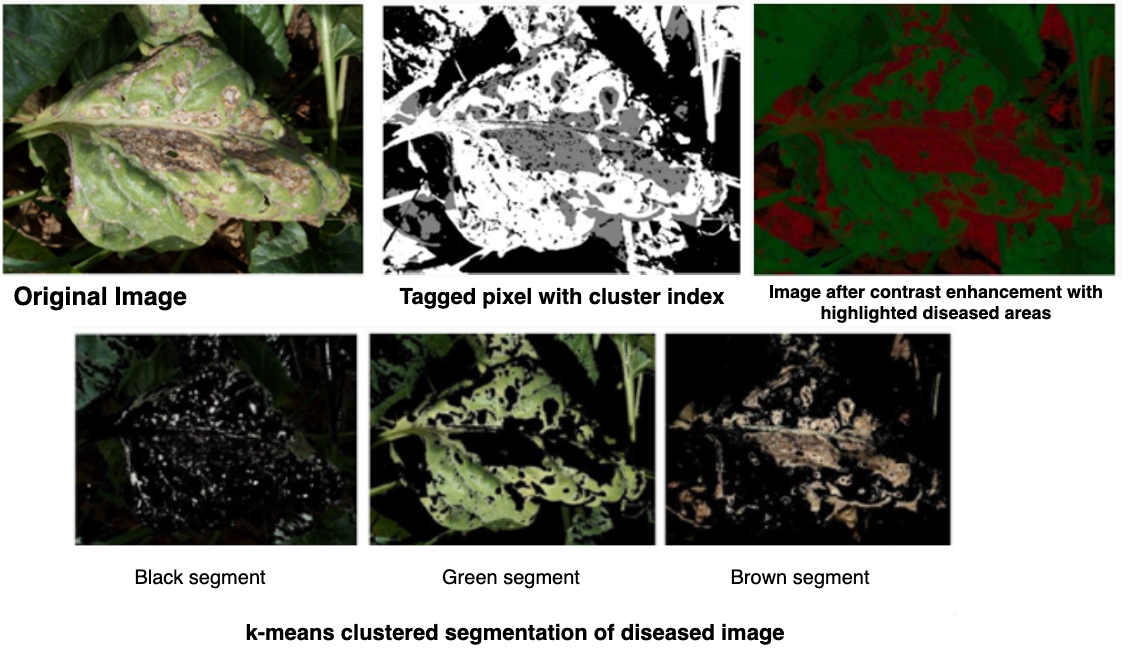
\includegraphics[scale=0.32]{figure/Untitled.png}}
        \caption{Resulting image of each steps in the proposed techniques described in \cite{ziya34determination}.}

        \label{fig:k_clusterd}
    \end{figure}


\item Bauer et al. \cite{bauer2011potential} in their paper researched the potential of using  KNN and adaptive Bayes with GMM pixel-wise algorithms to classify leaf disease in sugar beets automatically. They also investigated the use of conditional random fields (CRF) global labelling approach to improving pixel-wise-based classification results. Their classification task had three classes: $healthy \thinspace leaf \thinspace area$, $Cercospora \thinspace beticola$, and $Uromyces \thinspace betae$. For their experimental purpose, the authors inoculated 15 plants with the leaf spot pathogen $Cercospora \thinspace beticola$ and another 15 plants with the rust fungus $Uromyces \thinspace betae$. For each of the four leaves in each plant, they took 4 RGB images (FujiFilm FinePix S5600, 2592 x 1944) and one multispectral image (Tetracam ADC, 1280 x 1024, wavelength 700 - 950 nm) from a height of 30 cm and at different positions separated by about 10 cm. Then, they fused the five images of each leaf into one image representing the 3-D structures of the combined leaves’ to allow for rectification. The rectification of the 3-D image resulted in a 15-channel 2-D image. From these 15 values, they used only one blue, one green and one red value from one of the RGB images and the infrared channel from the multispectral image as classification features. They selected image patches that showed only healthy and infected leaf areas with no background for training and testing their models. From the resulting image patches, they chose 350 randomly for both diseases so that the test dataset finally contained 700 image patches. Also, in training their kNN classifier, they performed two experiments. The first experiment trained using four colour information from a particular pixel and the other using neighbouring pixels. For each experiment, they randomly chose 2000 pixels from half of the  700 image patches in the test dataset for training, and the other half was used for testing purposes. This was done to reduce the training computation time, and the kNN training and testing were done five times for each experiment. Likewise, They trained their adaptive Bayes classification models using Gaussian mixture models. 1 in 10 of the 700 image patches was randomly selected and used their complete information for training.
The trained model was then tested on the remaining 630 image patches. Thus, the GMM model training and testing were done ten times. Their kNN classifier achieved median accuracies of 84\%, 74\%, and 59\% for the $healthy \thinspace area$, $Cercospora \thinspace beticola$ and $Uromyces \thinspace betae$ respectively from the first experiment. In contrast, the median classification achieved in the second experiment were 91\%, 81\% and 76\% for the $healthy \thinspace area$, $Cercospora \thinspace beticola$ and $Uromyces \thinspace betae$ respectively. Likewise, the median accuracies for GMM trained models were 94\% for the $healthy \thinspace leaf \thinspace area$, 91\% for $Cercospora \thinspace beticola$ disease and 91\% for $Uromyces \thinspace betae$ disease. Finally, their CRF experiments concluded that it is possible to improve the result of an independent pixel-wise classifier with a global smoothing model. Likewise, their best classifier (GMM) results concluded that differentiating between healthy and infected sugar beet leaves is possible.
\end{enumerate}

\begin{table}[h!]
\centering 
 \begin{tabular}{p{2cm}|p{2cm}|p{2cm}|p{2cm}|p{2cm}|p{2cm}} 
%   \begin{tabular}{|c|c|c|c|c|}
 \hline
  Sensor & Wavelength & No. of Images Used & Model & Overall Accuracy & Reference\\ [0.5ex] 
 \hline\hline
 hand-held VIS-NIR spectrometer & 400 - 1000 nm & 50 & KNN, PLS, RF, SVML, SVMR & -  & \cite{Barreto2020HyperspectralIO} \\ 
 \hline
 RGB imaging (Smartphones) & - & 495 & SVM & 94.6\% & \cite{hallau2018automated} \\ 
 \hline
 RGB imaging (Nikon D300) & - & - & SVM & 99.47\% & \cite{zhou2013early} \\ 
 \hline
  RGB imaging (DJI Phantom 3) & - & 12 & KNN & - & \cite{ziya34determination} \\ 
 \hline
  RGB imaging (FujiFilm FinePix S5600) \& multispectral imaging (Tetracam ADC) & 700 - 950 nm & 700 & KNN, GMM & 91\%, 94\% & \cite{bauer2011potential} \\ 
 \hline

 \end{tabular}
 \caption{Overview of researches using machine learning algorithms for leaf disease detection in sugar beet.}
 \label{table:3}
\end{table}

\FloatBarrier

The studies in this chapter explored non-invasive leaf disease detection techniques in sugar beet with different ML and DL learning-based approaches. These studies demonstrate that sugar beet plant leaves can be monitored and classified as healthy or infected based on hyperspectral and RGB imaging data. Table \ref{table:2} shows an overview of the key metrics in the reviewed machine learning-based research papers, while table \ref{table:3} shows CNN learning-based approaches. The hyperspectral images provide spectral information that enables disease detection using learning-based algorithms. In contrast, the colour channels in RGB images give enough information for leaf disease detection and classification tasks.
    
   

